\chapter{Lập trình cơ bản NodeJS}
\label{ch: Lập trình cơ bản NodeJS}

\section{Một số module làm việc vào ra}
		Node cung cấp một số module làm việc trực tiếp với file.
	\subsection{Module fs}
		Đây là module chính giúp ta có thể thao tác với tệp.Module này cung cấp các thao tác tệp bao gồm:
		\begin{itemize}
			\item Tạo lập, đổi tên, xóa tệp 
			\item Thao tác trên tệp: mở tệp, đọc, ghi, đóng tệp 
			\item Cập nhật thời gian truy cập
			\item Thay đổi quyền sở hữu và quyền truy cập (trên hệ thống linux)
			\item …
		\end{itemize}
		
		Một điểm chú ý là NodeJS hỗ trợ asynchronous IO và synchronize IO với thao tác tệp. Ta dễ dàng nhận biết các lệnh này thông qua tên gọi. Các lệnh đọc file đồng bộ sẽ có 'Sync' trong tên. Ví dụ:
		\begin{itemize}
			\item readFile(filename: string, data: mixed, [encoding], [callback:function])
			\item readFileSync(filename: string, data: mixed, [encoding], [callback: function])
		\end{itemize}
		
		Ta cũng có thể kiểm tra thông tin về trạng thái tệp, thư mục nhờ module này. Một số hàm kiểm tra trạng thái. 
		\begin{itemize}
			\item fs.stat(filename: string, callback: function) : đọc thông tin trạng thái, khi đọc xong gọi hàm callback. Tham số hàm callback bao gồm lỗi (nếu có) và object chứa thông tin về file
			\item Các hàm kiểm tra kiểu file: Kiểm tra các kiểu file . Các kiểu file này tương ứng trong hệ thống POSIX:
			\begin{itemize}
				\item isFile();
				\item isDirrectory(): kiểm tra loại file là thư mục.
				\item isBlockDevice(): kiểm tra loại file là thiết bị block.
				\item isCharacterDevice(): kiểm tra thiết bị thuộc loại đọc ký tự.
				\item isSymbolicLink(): file là link.
				\item isFIFO(): thiết bị đọc dạng FIFO.
				\item isSocket(): socket.
			\end{itemize}
			
		\end{itemize}

	\subsection{Module path}

		Module này chứa các tiện ích giúp xác định và biến đổi đường dẫn của tệp. Một số phương thức chính:
		\begin{itemize}
			\item resolve: xác định địa chỉ tuyệt đối file dựa trên địa chỉ tương đối tệp đó với một địa chỉ tuyệt đối
			\item join: nối địa chỉ với nhau
		\end{itemize}
		
		\begin{figure}[-h]
			\centering
			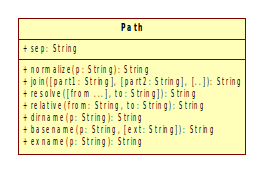
\includegraphics[scale=0.7]{3_3_0}
		\end{figure}

%================== Một số module về mạng ===================
\section{Một số module về mạng}
	\subsection{HTTP \& HTTPS}
	Module HTTP là tập hợp các thao tác qua mạng . Module này gồm có các lớp:
		\begin{itemize}
			\item http.Server: lớp server
			\item http.ServerRequest : cho phép biểu diễn thông tin truy vấn tới server.
			\item http.ServerResponse : lớp biểu diễn các thông tin trả về từ server.
			\item http.ClientRequest: lớp biểu diễn yêu cầu dữ liệu.
		\end{itemize}	
		
		\begin{figure}[h]
	    	\centering
			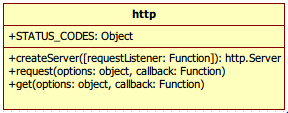
\includegraphics[scale=0.7]{3_3_1}
		\end{figure}		 
		
		HTTP là một trong những thành phần quan trọng nhất giúp Nodejs hoạt động như một Web Server. HTTP module cung cấp phương thức createServer giúp tạo ra một thể hiện của lớp HTTP Server. Ngoài ra có một số sự kiện và cấu trúc dữ liệu để thực hiện các callback.
		
	\subsubsection{http.Server}
		
		\begin{figure}[h]
			\centering
			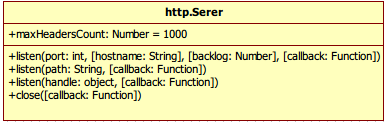
\includegraphics[scale=0.7]{3_3_2}
		\end{figure}
		
		Phương thức listen trong lớp này thiết lập thông tin cho server như cổng, tên host, đường dẫn,.. Phương thức close nhằm đóng lại server. Ngoài ra một http Server sẽ có các sự kiện cơ bản sau:
		
		\begin{itemize}
			\item 'request' : Sự kiện sẽ được kích hoạt mỗi khi có một yêu cầu (request) tới server. Tham số của hàm callback gồm :
				\begin{itemize}
					\item req : một thể hiện của lớp http.serverRequest, chứa thông tin yêu cầu từ máy client
					\item res : một thể hiện của lớp http.serverResponse, chứa thông tin trả về do máy chủ tạo ra
				\end{itemize}
			\item 'connection': Sự kiện được kích hoạt khi có một luồng dữ liệu TCP xuất hiện. Chú ý rằng với một liên kết TCP có thể gồm nhiều request.
			\item 'close': Khi server đóng
			\item 'checkContinue': Sự kiện được kích hoạt khi có 100  kết nối liên tiếp. Mục đích của sự kiện này giúp lập trình viên tăng khả năng điều khiển . Mặc định, nếu sự kiện này không được cài đặt, 100 kết nối này sẽ được đáp ứng.
			\item 'connect' : Sự kiện được kích hoạt khi có một kết nối http CONNECT .Nếu sự kiện này không được  lắng nghe, mặc định các kết nối sẽ bị đóng lại. Tham số truyền vào callback gồm:
			\begin{itemize}
				\item request: tham số của request.
				\item socket: socket giữa server và client.
				\item head: một thể hiện của lớp Buffer, gói đầu tiên của .., thường được để trống.
			\end{itemize}

			\item 'upgrade' : sự kiện được kích hoạt khi client có yêu cầu http upgrade.
			\item 'clientError': sự kiện được kích hoạt khi kết nối server và client thất bại.
		\end{itemize}
		
	\subsection{Lớp http.ServerRequest}
		
		Lớp này được tạo ngầm định bởi server, được truyền như một tham số như ta đã thấy trong sự kiện 'request' của một Server. Lớp này thực thi giao diện của Readable Stream kế thừa EventEmitter. Các sự kiện cơ bản của lớp này :
		\begin{itemize}
			\item 'data': sự kiện được kích hoạt khi nhận được các đoạn tin. Các đoạn tin này là một xâu nếu kiểu mã hóa xác định thông qua phương thức setEncoding hoặc một Buffer nếu không xác định.
			\item 'end': sự kiện được kích hoạt với ý nghĩa không còn gói tin nào nữa
			\item 'close': sự kiện báo đóng kết nối
		\end{itemize}
		
		\begin{figure}[h]
			\centering
			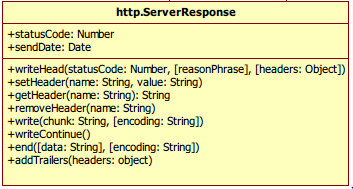
\includegraphics[scale=0.7]{3_3_3}
		\end{figure}

		Ngoài ra lớp này còn một số trường giúp cung cấp thêm các thông tin về request:
		\begin{itemize}
			\item method: phương thức yêu cầu : GET/POST/..
			\item url:  xâu biểu diễn các yêu cầu (ví dụ: '?id='1'\& type=2')
			\item httpVersion: phiên bản version
			\item trailer: HTTP trailers
			\item headers: đối trượng chứa tất cả các thông tin trường header của request
		\end{itemize}
		
		\begin{figure}[h]
			\centering
			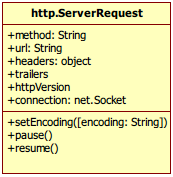
\includegraphics[scale=0.7]{3_3_4}
		\end{figure}				
		
	\subsubsection{Lớp http.serverResponse}
		Đây là lớp được tạo ra do server khi có sự kiện 'request'. Cấu trúc lớp nà được thể hiện như hình bên. Trong đó, một số phương thức quan trọng:
		\begin{itemize}
			\item writeHeader: thiết lập thông tin header trả về cho client
			\item write : viết thông tin trả dữ liệu trả về cho client.
			\item End : tín hiệu báo  đã truyền xong dữ liệu cho server
		\end{itemize}
		
		\begin{figure}[h]
			\centering
			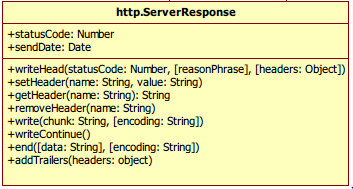
\includegraphics[scale=0.7]{3_3_5}
		\end{figure}
		
		
	\subsubsection{http Client}		
			
		Một trong các đặc điểm quan trọng của Nodejs là phía server có thể thực hiện các yêu cầu HTTP tới các địa chỉ khác như một máy khách. Điều này đặc biệt hữu ích trong trường hợp muốn duy trì kết nối giữa các server.
		
		Để tạo một yêu cầu HTTP ta thực hiện thông qua lệnh : 
		
		\begin{minted}[linenos=true, tabsize=4]{javascript}
http.request(options: String, callback: function);
		\end{minted}
		
	Options là một xâu hoặc một đối tượng. Trong trường hợp là đối tượng nó sẽ được tự động chuyển thông qua hàm url.parse(). Một số tùy chọn cho option:
	\begin{itemize}
		\item host: tên miền hoặc IP muốn kết nối đến. Mặc định, tên miền là 'localhost'
		\item port: cổng kết nối
		\item method: phương thức HTTP (GET, POST,..). Mặc định phương thức kết nối là 'GET'
		\item path: đường dẫn yêu cầu
		\item headers: các thông tin headers
		\item Agent:  user-agent của máy. Đây là một thể hiện của lớp http.Agent
	\end{itemize}
	Ví dụ sau minh họa cho việc thực hiện một yêu cầu tìm kiếm tới Google:
	
	\begin{minted}[linenos=true, tabsize=4, frame=single]{javascript}
var http = require('http');
var query = ' Nodejs Information';
var opts = {
	host : 'google.com',
    port : 80,
    path: '/search?q=' + query,
    method: 'GET'
};

var req = http.request(opts, function(res){
	console.log(res); //display response information 
    res.setEncoding('utf8');
    res.on('data', function(data){
		console.log(data);
    }
});

req.end(); //send request
	\end{minted}
	
	Đây là kết quả khi thực hiện xong chương trình:
	Ngoài ra bạn cũng có thể sử dụng http.get() trong trường hợp phương thức HTTP chỉ là GET, cách sử dụng cũng tương tự như trên.
	\begin{figure}[-h]
		\centering
		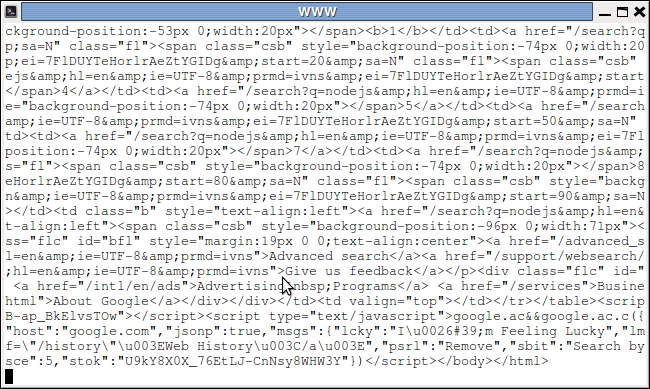
\includegraphics[scale=0.7]{3_3_6}
	\end{figure}
	
\newpage
	
%=========================================
\subsection{Net}
	Module net là lớp bao của module http. Module này cho phép thiết lập và tạo các TCP server. Nó chứa đựng các phướng thức cho việc tạo cả một server và client. Chúng ta có thể sử dụng module này với \textbf{require('net');}\\
Một số phương thức của module Net:
        \subsubsetion{net.createServer([options], [connectionListener])}
        Tạo ra một TCP server mới. Thamm số connectionListener được tự động thiết lập việc bắt sự kiện "connection". options là một đối tượng với mặc định \\
            \begin{minted}[linenos=true, frame=single, tabsize=true]{javascript}
var net = require('net');
var server = net.createServer(function(c) { //'connection' listener
  console.log('server connected');
  c.on('end', function() {
    console.log('server disconnected');
  });
  c.write('hello\r\n');
  c.pipe(c);
});

server.listen(8124, function() { //'listening' listener
  console.log('server bound');
});
            \end{minted}
        \\    
      \subsubsection{net.connect(options, [connectionListener])}
      \subsubsection{net.createConnection(options, [connectionListener])} 
      Xây dựng một đối tượng socket mới và mở socket nhất định. Khi socket được thành lập, sự kiện 'connect' sẽ được sinh ra.
      
      Với TCP sockets, đối số options được đối tượng đăc tả:
        \begin{itemize}
            \item \textbf{port}: Port của client để kết nối (Required).
            \item \textbf{host}: Host của client để kết nối tới, mặc định là 'localhost'.
            \item \textbf{localAddress}: Giao diện địa phương để ràng buộc các kết nối.
        \end{itemize}

Đây là một ví dụ:
    \begin{minted}[linenos=true, frame=single, tabsize=4]{javascript}
var net = require('net');
var client = net.connect({port: 8124},
    function() { //'connect' listener
  console.log('client connected');
  client.write('world!\r\n');
});

client.on('data', function(data) {
  console.log(data.toString());
  client.end();
});

client.on('end', function() {
  console.log('client disconnected');
});   
    \end{minted}
    
    \\
    \subsubsection{net.connect(options, [host], [connectionListener])}
    \subsubsection{net.createConnection(options, [host], [connectionListener])}
        Tạo ra một TCP kết nối từ \texttt{port} trong \texttt{host}. Nếu \texttt{host} bị bỏ qua, \texttt{'localhost'} sẽ được chọn giả định. Tham số connectListener sẽ được thêm vào như việc bắt sự kiện cho sự kiện \texttt{"connect"}
     
     \\
     \subsubsection{net.connect(path, [connectListener])}
     \subsubsection{net.createConnection(path, [connectListener])}
        Tạo ra unix socket kết nối theo \texttt{path}. Tham số connectListener sẽ được thêm vào như việc bắt sự kiện cho sự kiện \texttt{"connect"}.
%=========================================
\subsection{URL \& QueryString}
	Đây là 2 module tiện ích hỗ trợ cho việc xử lý URL và các truy vấn. \\
	Module URL giúp cho việc xử lý URL. Với module này ta có thể tách xâu URL thành đối tượng biểu diễn thông tin: host, hostname, querystring... \\
	URL cung cấp 3 phương thức để xử lý xâu:
		\begin{itemize}
			\item parse: Chuyển từ xâu truy vấn thành một đối tượng chứa thông tin về url. Các thông tin đó gồm:
			\begin{itemize}
				\item protocol : giao thức kết nối
				\item hostname : tên host, sử dụng khi không có thông tin trường host
				\item host: thay thế cho hostname và port
				\item pathname: đường dẫn
				\item search:  thành phần biểu diễn yêu cầu nội dung tìm kiếm là query
				\item query: nội dung tìm kiếm
				\item hash: phần thông tin bắt đầu bởi dấu \#
			\end{itemize}
			\item format: chuyển từ đối tượng thành url
			\item resolve(baseURL: String, href: String) : xây dựng xâu biểu diễn url từ 2 thành phần based URL và href. Ví dụ ta có xâu cơ bản "\url{http://google.com/test}" và href là "/search?q=nodejs", xâu trả về sẽ là "\url{http://google.com/search?q=nodejs}" 
		\end{itemize}
	Ta có ví dụ cho việc chuyển đổi xâu truy vấn:\\
	
	\begin{figure}[h]
		\centering
		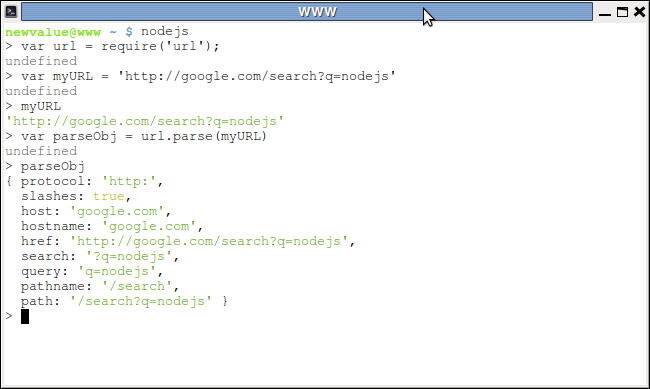
\includegraphics[scale=0.7]{3_3_7}	
	\end{figure}

	Lớp QueryString cung cấp các công cụ giúp  xử lý xâu truy vấn. Lớp này cung cấp một số phương thức cơ bản sau:\\
	
	\begin{itemize}
		\item \textbf{stringify(obj: Object, [sep: String], [eq])} : Chuyển một đối tượng biểu diễn truy vấn thành một xâu. Mặc định Node sử dụng dấu ngăn cách giữa các truy vấn là dấu '\&' và biểu diễn gán giá trị bằng dấu '='. Ta có thể tùy chỉnh các dấu này nếu cần
		\item \textbf{parse(str,[sep: String],[eq: String],[options: Object])}: Chuyển xâu thành đối tượng biểu diễn truy vấn
		\item \textbf{phương thức escape() và unescape()}: 2 phương thức này hoạt động như phương thức stringify và parse nhưng có thể được ghi đè nếu cần thiết.
	\end{itemize}
	
	Ta có ví dụ sau:\\
	
	\begin{minted}[linenos=true, tabsize=4, frame=single]{javascript}
querystring.parse('foo=bar&baz=qux&baz=quux&corge')

// returns

{ foo: 'bar', baz: ['qux', 'quux'], corge: '' }

querystring.stringify({ foo: 'bar', baz: ['qux', 'quux'], corge: '' })

// returns

'foo=bar&baz=qux&baz=quux&corge='
		
	\end{minted}
	
\subsection{DNS}
	Chức năng module này là giúp phân giải tên miền từ tên miền sang địa chỉ IP và ngược lại. Module này hỗ trợ cả phân giải dựa trên IPV4 và IPV6.
	\begin{figure}[-h]
		\centering
		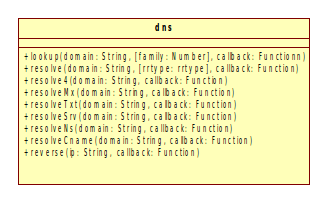
\includegraphics[scale=0.7]{3_3_8}
	\end{figure}
	

%========================= Một số module công cụ =====================
\section{Một số module công cụ}
	\subsection{Console}
	Đây là module toàn cục, tức ta không cần phải nạp module để chạy được các hàm mà nó cung cấp. Module này cung câp một đối tượng 'console' giúp ta có thể in ra các thông tin. Ví dụ:
	\begin{minted}{javascript}
console.log('hello world');
	\end{minted}

	Trong trường hợp muốn ghi thông báo lỗi, ta sử dụng lệnh warn:\\
	\begin{minted}{javascript}
console.warn('Đang có lỗi gì đó :)');
	\end{minted}

	Để in dấu vết, ta dùng hàm :
	\begin{minted}{javascript}
console.trace();
	\end{minted}
%================================= Util ==================================
	\subsection{Util}
		Module này chức năng tương tự như console nhưng mạnh mẽ hơn. Một số hàm thông dụng:
		\begin{itemize}
			\item util.format(format,[]): định dạng văn bản hiển thị ra tương tự như hàm printf trong C
			\item util.debug(string: str): block tiến trình hiện tại và in xâu str ra stderr
			\item util.inspect(obj: object, [option: object]): 	 trả về biểu diễn xâu của đối tượng. Đây là một công cụ hữu hiệu trong trường hợp muốn debug thông tin.Một số tùy chọn khi gọi hàm này:
			
			\begin{itemize}
				\item showHidden: thiết lập hiển thị với các đối tượng không có tính chất liệt kê
				\item depth: giới hạn độ xâu kiểm tra
				\item colors: hiển thị màu sắc cho kết quả
			\end{itemize}
			
			\item util.isArray:  dùng để kiểm tra đối tượng truỳen vào có phải là một mảng hay không		
		\end{itemize}

%================================ Event Emitter ===================================
	\subsection{Event Emitter}
	Trong Node có nhiều đối tượng có thể sinh ra nhiều sự kiện. Chẳng hạn như, một TCP server có thể sinh ra  một sự kiện "connect" trong mỗi lần mấy client kết nối tới. 
		\subsubsection{emitter.addListener(event, listener)}
		\subsubsection{emitter.on(event, listener)}
Thêm một listeners vào cuối mảng listener cho sự kiện được đặc tả.
			\begin{minted}[linenos=true, frame=single, tabsize=4]{javascript}
server.on('connection', function (stream) {
  console.log('someone connected!');
});
			\end{minted}
			
			
		\subsubsection{emitter.once(event, listener)}
Nếu muốn bắt sự kiện về  liên kết tới server, bạn sử dụng: 
			\begin{minted}[linenos=true. frame=single, tabsize=4]{javascript}
server.once('connection', function (stream) {
  console.log('Ah, we have our first user!');
});
			\end{minted}
		
		\subsubsection{emitter.removeListeners(event, listener)}
		Gỡ bỏ một listener từ mảng listener mà đặc tả cho sự kiện.
		    \begin{minted}{javascript}
var callback = function(stream) {
  console.log('someone connected!');
};
server.on('connection', callback);
// ...
server.removeListener('connection', callback);		    
		    \end{minted}
			
	    \subsubsection{emitter.removeAllListener([event])}
		Nếu bạn cần, bạn có thể gỡ bỏ việc bắt sự kiện từ Event Emitter bởi một lời gọi đơn giản\\
			\begin{minted}[linenos=true]{javascript}
server.removeAllListeners('connection');
			\end{minted}

\subsubsection{Tạo một Event Emitter}
			\begin{minted}[linenos=true, frame=single, tabsize=4]{javascript}
var EventEmitter = require('events').EventEmitter,
	util 		 = require('util');

// Here is the MyClass Contructor
var MyClass = function(option1, option2) {
	this.option1 = option1;
	this.option2 = option2;
}

util.inherits(MyClass, EventEmitter);
			\end{minted}
			
	Trong trường hợp của này, MyClass có thể sinh ra các sự kiện:\\
	\begin{minted}[linenos=true, frame=single, tabsize=4]{javascript}
MyClass.prototype.someMethod = function() {
	this.emit('custom event', 'some arguments');
}
	\end{minted}
	
	\begin{minted}[linenos=true, frame=single, tabsize=4]{javascript}
var myInstance = new myClass(1, 2);
myInstance.on('custom event', function() {
	console.log('got a custom event!');
});
	\end{minted}
%================================= Buffer ==================================
	\subsection{Buffer}
		Buffer là đối tượng cơ bản quan trọng nhất trong NodeJS. Khi truyền dữ liêu qua mạng, dữ liệu được xử lý dưới dạng nhị phân. Tuy nhiên, trong ngôn ngữ Javascript mặc định không có kiểu dữ liệu này. NodeJS đã thêm kiểu dữ liệu này. Khi dữ liệu gửi đến, mặc định là dữ liệu nhị phân. Để có thể chuyển sang dữ liệu văn bản, cần thiết lập kiểu mã hóa của văn bản. Ví dụ nếu văn bản mã hóa utf8, ta cần phải xác định kiểu mã hóa:\\
		\begin{minted}[linenos=true]{javascript}
	buf.setEncoding('utf8');
		\end{minted}
		
		Để khởi tạo một Buffer từ xâu, ta làm như sau:\\
		\begin{minted}[linenos=true]{javascript}
	buf = new Buffer(str: string, [encoding]);
		\end{minted}
		
		Ví dụ ta muốn tạo Buffer biểu diễn xâu "hello world" :
		\begin{minted}[linenos=true]{javascript}
	var buf = new Buffer("hello world");
		\end{minted}
		
		Trên kiểu Buffer ta có một số phương thức sau:
		\begin{itemize}
			\item \textbf{write(string: string, [offset: Number], [length: Number], [encoding: string])}: ghi dữ liệu vào xâu. \\
				\begin{minted}[linenos=true, tabsize=4, frame=single]{javascript}
buf = new Buffer(256);
len = buf.write('\u00bd + \u00bc = \u00be', 0);
console.log(len + " bytes: " + buf.toString('utf8', 0, len));				
				\end{minted}

			\item \textbf{toString([encoding],[start], [end])}: Trả về xâu biểu diễn Buffer tương ứng.
			\item \textbf{toJSON()}: trả về đối tượng JSON. \\
				\begin{minted}[linenos=true, frame=single, tabsize=4]{javascript}
var buf = new Buffer('test');
var json = JSON.stringify(buf);

console.log(json);
// '[116,101,115,116]'

var copy = new Buffer(JSON.parse(json));

console.log(copy);
// <Buffer 74 65 73 74>

				\end{minted}
			\item \textbf{byteLength(string: string, [encoding])}: trả về độ dài xâu \\
				\begin{minted}[linenos=true, tabsize=4, frame=single]{javascript}
// example byteLength method
str = '\u00bd + \u00bc = \u00be';

console.log(str + ": " + str.length + "characters, " +
	Buffer.byteLength(str, 'utf8') + " bytes");
				\end{minted}

			\item \textbf{concat(list: array, [totalLength: Number])}: Nối các buffer vào buffer cũ.
			\item \textbf{slice([start:Number],[end: Number])}: Trả về một Buffer mới. Buffer này  tham chiếu đến cùng vùng nhớ với Buffer cũ nhưng bị giới han bởi chỉ số start và end. \\
				\begin{minted}[linenos=true, frame=single, tabsize=4]{javascript}
var buf1 = new Buffer(26);

for (var i = 0 ; i < 26 ; i++) {
  buf1[i] = i + 97; // 97 is ASCII a
}

var buf2 = buf1.slice(0, 3);
console.log(buf2.toString('ascii', 0, buf2.length));
buf1[0] = 33;
console.log(buf2.toString('ascii', 0, buf2.length));
				\end{minted}
			\item \textbf{fill(value: Number,[offset: Number],[end: Number])}: điền đầy Buffer với dữ liệu value.\\
				\begin{minted}[linenos=true, frame=single, tabsize=4]{javascript}
var b = new Buffer(50);
b.fill("h");
				\end{minted}
		\end{itemize}
		
